%%%%%%%%%%%%%%%%%%%%%%%%%%%%%%%%%%%%%%%%%%%%%%%%%%%%%%%%%%%%%%%%%%%%%%%%%%%%%%%%
% Nationalsången (Du gamla, du fria)
%%%%%%%%%%%%%%%%%%%%%%%%%%%%%%%%%%%%%%%%%%%%%%%%%%%%%%%%%%%%%%%%%%%%%%%%%%%%%%%%

%###############################################################################
% Elias Hachichou, F13, 180316
%###############################################################################

% Hej! Vad kul att du vill hjälpa till med sångboken!
% Denna mall skall vägleda dig i hur du ska lägga in sånger i .tex!
% Till din hjälp behöver du en texteditor. Oavsett operativsystem så
% bör du ha en tillgänglig med jag rekommenderar Atom Texteditor som går 
% att ladda ner gratis. 
% Starta texteditorn och skapa en ny fil som du döper till sångnamnet
% använd endast små bokstäver och a-z. Använd understreck istället för 
% mellanslag.
% Filen skall sparas i .tex format. Om du använder Atom så kommer
% programmet att automatiskt att färgkoda koden.
% Jag rekommenderar att kopiera innehållet i denna fil och att sedan
% arbeta utifrån det.
% När du är färdig så skall det se ut som i internationalen.tex
% Alla kommentarer skall vara borta och avgränsare skall finnas.
% Du får lägga in ditt namn, på samma sätt som ovan.
% Lycka till!

% Här skall du sätta in en genomsnittligt lång rad från sången. Detta för att veta hur texten ska centreras under kompileringen.
\settowidth{\versewidth}{Din sol, Din himmel, Dina ängder gröna,}

% Sångtitel, här skriver du in sångtiteln
\poemtitle{Nationalsången (Du gamla, du fria)}

%------------------------------------------------

\begin{verse}[\versewidth]

% Här skriver du in vilken melodi som används (glöm inte att ta med "Mel."!)
\flagverse{}
\emph{Mel. Folkmelodi från Västmanland}\\!

%------------------------------------------------

% Flagverse numrerar verserna. Om sången innehåller refränger så hänvisar jag till det format som används i internationalen.tex
% Se även pdf:en för vägledning
% \\ avslutar en rad, * förhindrar sidbrytning efter den raden
% ! markerar styckesslut (obs. det får bli sidbrytning efter styckesslut)
\flagverse{1.}
Du gamla, Du fria, Du fjällhöga nord\\*
Du tysta, Du glädjerika sköna!\\*
Jag hälsar Dig, vänaste land uppå jord,\\*
/:Din sol, Din himmel, Dina ängder gröna.:/\\!

%------------------------------------------------

\flagverse{2.}
Du tronar på minnen från fornstora dar,\\*
då ärat Ditt namn flög över jorden.\\*
Jag vet att Du är och Du blir vad du var.\\*
/:Ja, jag vill leva jag vill dö i Norden.:/\\!

%------------------------------------------------

% Författare, om författare ej är känd så bortse från detta. Årtal är ej nödvändigt.
\poemauthorcenter{Richard Dybeck, 1844}

%------------------------------------------------

% Grafik. All grafik skall vara i svartvitt och måste vara i .png .jpeg eller .pdf format
% Bredden skall vara densamma i hela sångboken (0.5\textwidth). Se till att inte ha
% för stora marginaler kring bilden, utan beskär den gärna om det skulle behövas.
% Grafik är ej nödvändigt. Om grafik ej skall användas så skall hela detta stycke tas bort.
\begin{figure}[H]
    \centering
    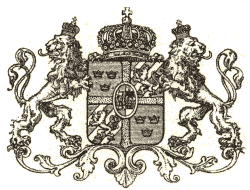
\includegraphics[width=0.5\textwidth]{riksvapnet.png}
\end{figure}

%------------------------------------------------

\flagverse{3.}
Jag städs vill dig tjäna, mitt älskade land,\\*
Dig trohet till döden vill jag svära.\\*
Din rätt skall jag värna med håg och med hand,\\*
/:Din fana, högt den bragderika bära.:/\\!

%------------------------------------------------

\flagverse{4.}
Med Gud skall jag kämpa för hem och för härd,\\*
för Sverige, den kära fosterjorden.\\*
Jag byter Dig ej mot allt i en värld\\*
/: Nej, jag vill leva jag vill dö i Norden!.:/\\!

%------------------------------------------------

% I detta fall finns det två författare därav denna rad.
\poemauthorcenter{Louise Ahléns, 1910}

%------------------------------------------------

% Obligatorisk
\end{verse}

%----------------------------------------------------------------------------------------